\documentclass[conference]{IEEEtran}
\hyphenation{OpenAi GPT-J}
\usepackage{svg}
\usepackage{float}
\usepackage{tikz}
\usepackage{makecell}
\usepackage{url}
\def\UrlBreaks{\do\/\do-}
\usepackage{breakurl}
\usepackage[breaklinks]{hyperref}
\usepackage{lipsum}  
\usepackage{listings}

\lstdefinelanguage{json}{
    basicstyle=\normalfont\ttfamily,
    numbers=left,
    numberstyle=\scriptsize,
    stepnumber=1,
    numbersep=8pt,
    showstringspaces=false,
    breaklines=true,
    frame=lines
}


\begin{document}
\begin{titlepage}
	\centering
	
\includegraphics[width=0.2\textwidth]{logoBlackV.eps}\par
	\vspace{1.5cm}
	{\LARGE Southern Adventist University \par}
	\vfill
	{\Large Senior Project\par}
	\vspace{1cm}
	{\huge\bfseries Algorithmically Trading like a Human with GPT-J\par}
	\vspace{1cm}
	{\large Joel \textsc{Peckham}\par}
	\textsc{Email:} \href{mailto:joelskyler@gmail.com}{joelskyler@gmail.com}\par
	
	\vspace{0.5cm}
	supervised by\par
	Willard \textsc{Munger}, PhD.\par
	Robert \textsc{Ordóñez}, M.S.
	\vfill
	\begin{abstract}
		% \lipsum[1]
		We explore the viability of using GPT-J, a 6 billion parameter natural language processing model, as a stock market trading indicator. This novel approach leverages both GPT-J's ability to process large, data-rich inputs, and GPT-J's deep understanding of the world. We study the viability of using GPT-J as a natural language based stock predection algorithm by creating and evaulating a small scale test dataset. Our test dataset produced no significant results. 
	\end{abstract}
	
	\vfill
	
	% Bottom of the page
	{\large \today\par}
\end{titlepage}
\onecolumn
\tableofcontents
\listoffigures
\listoftables
\twocolumn
\section{Introduction}
\subsection{Background}
Algorithmic trading has become the dominant way of buying and selling securities. In the U.S. stock market, algorithms account for 70-80\% of trading volume \cite{Samuelsson2021}. The current generation of trading algorithms now use neural networks to improve prediction accuracy. However, some believe neural networks are incapable of inventing novel trading ideas and therefore can only increase trading efficiency by approximately 10\% \cite{Vonko2021}. On the other hand, we propose that recent increases in the scale of neural networks can unlock the ability to algorithmically invent winning trades. 

Specifically, we propose that large-scale natural language processing models such as OpenAi's GPT-3 \cite{Brown2020} have captured a large enough understanding of the world, that given the proper input, they can generate novel, winning trades. Transformer networks of this type are designed to both ingest and output text. We propose that by properly engineering our input text prompts, we can leverage the massive amount of real-world knowledge encoded in the network's weights.

Because of the complications inherit in working with OpenAi and licensing GPT-3, we have instead chosen to use the open-source project GPT-J \cite{mesh-transformer-jax}. GPT-J is a transformer network \cite{Vaswani2017} that has been trained on an 825GiB language modeling data set called The Pile \cite{Gao2021}. Compared to GPT-3-Davinci's 175 billion network parameters, GPT-J's 6 billion parameters seems small, however it has proved itself to be capable enough to outperform GPT-3 in some tasks such as code generation \cite{forefront}. Therefore, we believe that GPT-J will be sufficient to explore the viability of our novel approach to trading.

Taking into account the impressive knowledge displayed by GPT-3 and others in text-completion tasks, we propose that with adequate fine-tuning and well engineered prompts, GPT-J can learn to trade like a human by reading the news, social media, and other sources such as SEC filings.

% \subsection{Intent}
% We will first implement a trading algorithm based on GPT-J. Then, we will evaluate the algorithm's prediction accuracy and compare it to the accuracy of similar algorithms. Optimizing our algorithm will involve multiple iterations of fine-tune network training, prompt engineering, and accuracy analysis. Finally, we will conduct a profitability analysis of our algorithm using back-testing and live data.

\subsection{Problem Statement}
As algorithmic traders seek to employ increasingly competitive and complex trading algorithms, we propose to study the viability of using GPT-J as a natural language based stock predection algorithm. This work will provide a foundation for developing and testing such an algorithm by building and evauluating a small-scale test dataset. 

\section{Review of Literature}
\subsection{Previous Methods}
Many neural network structures and methods have been used to create trading algorithms. Some types include: 
\begin{itemize}
	\item Recurrent neural networks (RNNs) \& Long short-term memory (LSTMs) \cite{Chen2017}\cite{Mehta2021}.
	      \\\emph{These are the most widely used network architectures for trading \cite{Gu2020}. An LSTM trained on 900,000 sequences of length 30 days of Chinese stock market data yielded an improvement of 12.9\% in prediction accuracy over a random guess \cite{Chen2015}.}
	\item Convolutional Neural Networks (CNNs) \cite{Gu2020}
	      \\\emph{CNNs can be used by converting time-series data into images \cite{Sezer2018}. Or they can be used to extract sentiment features from text \cite{Shi2020}.}
	\item Deep reinforcement learning (DRN).
	      \begin{itemize}
	      	\item Deep Q-learning \cite{Wang2017} \cite{Nan2020}.
	      	\item Deep robust reinforcement learning \cite{Li2019}.
	      \end{itemize}
	\item Conventional deep learning \cite{Day2016}.
	\item Transformer networks \cite{Schmitz2020}.
\end{itemize}

Most relevant to our work are methods that incorporate sentiment analysis of news sources. \cite{Mehta2021} evaluated sentiment analysis methods and found that LSTMs could correctly classify news tweets as indicative of positive or negative price movement 92\% of the time. \cite{Nan2020} found that adding sentiment analysis to a Deep-Q learning algorithm could improve the Sharpe Ratio (a measure of profit as compared to risk) of the agent by a factor greater than 2 in their test cases.

\subsection{Relevance \& Novelty}
By our estimation, the vast majority of previous works involving sentiment analysis used a pre-processing step to extract sentiment from the news, and then embedded those features into a time-series dataset. News sources were often limited to headlines, tweets and small snippets because of the memory limitations of RNN sentiment classifiers. With the introduction of large transformer networks \cite{Vaswani2017}, capable of processing large amounts of text like OpenAi's GPT-3 \cite{Brown2020} or Wang \& Komatsuzaki's GPT-J \cite{gpt-j}, we believe a new class of trading network can be created. Readily available implementations of GPT-J allow for inputs with up to 2048 input tokens or words. Our method will encode the current world state in a large text-input which combines sentiment, real-world facts, and stock price data into a single input. We believe that combining rich input information with the network's pre-existing understanding of the world, the network will be able to produce significantly better trading signals than previous methods.

\section{Execution Plan}
To guide our execution, we have outlined the goals, requirements, steps, and processes we intend to implement. 
\subsection{Requirements \& Goals}
\subsubsection{Functional requirements (user stories)}
\begin{itemize}
	\item As finance researchers, we want to quantify the ability of news releases, SEC filings, and social media posts to move stock prices.
	\item As AI researchers, we want to evaluate the viability of using GPT-J as a stock movement indicator so that we can understand the power of GPT-J to understand complex real-world interactions.
	\item As algorithmic traders, we want to evaluate the viability of using GPT-J as a stock movement indicator so that I can make more-informed trading decisions.
\end{itemize}
\subsubsection{Non-functional requirements}
Our overall flow of execution as outlined in figure \ref{fig:executionFlow} is as follows:
\begin{enumerate}
	\item[•] We will evaluate the correlations between the following items:
	      \begin{enumerate}
	      	\item The release of SEC filings for company X and large movements in the stock price of company X.
	      	\item The release of news stories mentioning company X and large movements in the stock price of company X.
	      	\item The posting of tweets or other social media posts mentioning company X and large movements in the stock price of company X.
	      \end{enumerate}
	\item[•] We will evaluate the best ways of formatting prompts for GPT-J to increase output accuracy and consistency across varying inputs. Some options might include:
	      \begin{enumerate}
	      	\item Providing a form for GPT-J to fill out appended to the end of the input data.
	      	\item Asking GPT-J a direct question appended to the end of the input data.
	      	\item Appending a universe current stock prices to the beginning of the input.
	      	\item Appending multiple news stories from the past days and weeks at the beginning of the input.
	      \end{enumerate}
	\item[•] We will deploy the best model from my previous evaluations and test it on live stock market data. We will compare the model's performance against market indices like the S\&P 500. 
\end{enumerate}

\begin{figure}[ht]
	\centering
	\scalebox{0.8}{
		\definecolor{lblue}{RGB}{220, 234, 240}
		\definecolor{dblue}{RGB}{0, 21, 79}
		\newcommand\bluebox[3]{\filldraw [draw=dblue,fill=lblue, line width=0.4mm] (#1-1.75,#2-0.75) rectangle (#1+1.75,#2+0.75) node[text=dblue, font=\footnotesize][midway] {\makecell[l]{#3}}}
		\newcommand\bluearrow[4]{\draw[dblue, -latex, line width=0.8mm] (#1,#2-0.75) -- (#3,#4+0.75);}
		\newcommand\bluearrownooffset[4]{\draw[dblue, -latex, line width=0.8mm] (#1,#2) -- (#3,#4);}
		\newcommand\blueline[4]{\draw[dblue, line width=0.8mm] (#1,#2) -- (#3,#4);}
		\begin{tikzpicture}
			\bluebox{0}{0}{\textbf{Gather test dataset}\\(SEC filings, news, social\\media, stock price data)};
			\bluebox{0}{-2}{\textbf{Evaluate correlations}\\\textbf{between media release}\\\textbf{\& price movement}};
			\bluebox{2}{-4}{\textbf{Change type of}\\\textbf{input media}};
			\bluebox{0}{-6}{\textbf{Fine-tune training}\\\textbf{on GPT-J}};
			\bluebox{2}{-8}{\textbf{Change format of}\\\textbf{input prompt}};
			\bluebox{0}{-10}{\textbf{Evaluate prediction}\\\textbf{accuracy}};
			\bluebox{0}{-12}{\textbf{Test and evaluate}\\\textbf{on live data}};
			\bluearrow{0}{0}{0}{-2};
			\bluearrow{-1}{-2}{-1}{-6};
			\bluearrownooffset{0.25}{-4}{-1}{-4};
			\bluearrow{-1}{-6}{-1}{-10};
			\bluearrownooffset{0.25}{-8}{-1}{-8};
			\bluearrow{0}{-10}{0}{-12};
			\blueline{1.75}{-10}{4.21}{-10};
			\bluearrownooffset{2.75}{-10}{2.75}{-8.75};
			\blueline{4.25}{-4.04}{4.25}{-10.04};
			\bluearrownooffset{4.29}{-4}{3.75}{-4};
			\blueline{2.75}{-7.25}{2.75}{-5.96};
			\bluearrownooffset{2.75}{-6}{1.75}{-6};
		\end{tikzpicture}
	}
	\caption{Execution Flow}
	\label{fig:executionFlow}
\end{figure}

\subsection{Dataset Gathering}
\subsubsection{Stock Price Data}
We plan to use the publicly available Yahoo Finance API \cite{yahoofinanceapi} to gather general technical information about a given ticker symbol. 
For historical price data, we will use the Alpaca Data API v2 \cite{alpacadataapi}. This API gives access to 5 years of historical data for training and live price data for live model inference testing. 
\subsubsection{SEC Filings}
The SEC provides public access to their EDGAR database of public company filings \cite{Sec.gov_2021}. The EDGAR API can be used to download the most recent SEC filings for a given company for live trading. Or for training, bulk datasets are available for download. The release dates of each filing can then be labeled with the stock prices of the company before and after the filing.
\subsubsection{News}
We will scrape financial news websites for a large set of historical articles. We intend to create a backlog of articles from the sources listed in Table \ref{table:newsSources}.
\begin{table}[ht]
    \caption{News Sources}
    \centering
    \begin{tabular}{|l|l|}
        \hline
        \textbf{Source} & \textbf{URL} \\
        \hline
        Bloomberg & \href{https://www.bloomberg.com/}{www.bloomberg.com} \\
        \hline
        CNBC Finance & \href{https://www.cnbc.com/finance/}{www.cnbc.com/finance} \\
        \hline
        Reuters & \href{https://www.reuters.com/}{www.reuters.com} \\
        \hline
        Forbes & \href{https://www.forbes.com/}{www.forbes.com} \\
        \hline
        CNN Business & \href{https://www.cnn.com/business}{www.cnn.com/business} \\
        \hline
        Yahoo Finance & \href{https://finance.yahoo.com/news}{www.finance.yahoo.com/news} \\
        \hline
        Wall Street Journal & \href{https://www.wsj.com/}{www.wsj.com/} \\
        \hline
    \end{tabular}
    \label{table:newsSources}
\end{table}

\subsubsection{Social Media}
We will focus on Twitter for our social media data. The Twitter API \cite{twitterapi} will allow us to gather timely opinions on a given ticker symbol. After filtering for a specific time period, tweets can be added to our training dataset.

\subsection{Testing \& Evaluation Methods}
\subsubsection{Media Release Correlations}
To measure the correlation between the release of a media item such as an SEC filing or news story, we will use the standard event study method as detailed in \cite{Neuhierl2010}. This method uses abnormal returns in a given period to calculate the effect of a certain event on a stock's price. Abnormal return for a given day is defined as 
\begin{equation}
	AR_{i,t}=R_{i,t}-(\alpha_i+\beta_i R_{m,t})
\end{equation}
for firm $i$ at time $t$ where $\alpha_i$ and $\beta_i$ represent the relationship between a given stock and it's reference market. And where $R_{m,t}$ is the return of the actual reference market. This method uses the historical relationship of a stock to it's reference market to estimate normal returns. Abnormal returns are therefore the difference between the actual return of the stock and the normal return of the stock. 

We can then take large sample of media release events of the same type and calculate the average abnormal return as follows:
\begin{equation}
	AAR= \frac{1}{N} \sum\limits_{i=1}^{N}AR_{i,t}
\end{equation}

Finally, we can measure the total impact of the event over a given period of time by using cumulative abnormal return:
\begin{equation}
	CAR(t_1,t_2)=\sum\limits_{t=t_1}^{t_2} AR_{i,t} 
\end{equation}
where $t_1$ and $t_2$ are the start and end dates of the event window.

Because we are limited in the granularity of data we have access to and can easily process, our research will focus on day-by-day events, returns, and correlations.

\subsubsection{GPT-J Model prediction accuracy}
To evaluate the accuracy of our model given different input data, we will use two metrics. First is a simple ratio of well-formed, parseable outputs to malformed outputs. This first metric we refer to as format-correctness. 
\begin{equation}
	F_c=\frac{N_{parseable}}{N_{malformed}}
\end{equation}
The second metric is a simple ratio of the actual stock price to the predicted stock price. This second metric we refer to as price-accuracy.
\begin{equation}
	P_a=\left|\frac{P_{actual}}{P_{predicted}}\right|
\end{equation}
We will use the price accuracy metric as our loss-function in fine-tune training of GPT-J. The format-correctness metric will be used to evaluate the reliability and robustness of our prompt. We may experiment with using the format-correctness metric as a weighted portion of our loss function.
\section{Implementation}
\subsection{Data Gathering}
We used a Digital Ocean droplet for data gathering and processing. This allowed us to dedicate a machine for long-running webscraping tasks and transfer data with a fast and reliable connection. 
\subsubsection{News Web Scraping}
Using the freely available New York Times Archive API {Citation Needed}. We downloaded the associated metadata for each New York Times article from January 2006 through October 2022. This subset of the New York Times archive consists of 1,446,289 articles. We then filtered the articles based on the keywords associated with the article, to get articles relevant to a company in our list of top 50 U.S. companies. Our resulting dataset contains 23428 unique articles from the Times. 

\begin{table}[ht]
    \caption{Stock Sources}
    \centering
\begin{tabular}{|l|l|}
	\hline
	\textbf{Company} & \textbf{Ticker} \\
	\hline
	Apple & AAPL \\
	Microsoft & MSFT \\
	Alphabet & GOOG \\
	Amazon & AMZN \\
	Facebook & FB \\
	Tesla & TSLA \\
	Berkshire Hathaway & BRK.A \\
	Nvidia & NVDA \\
	JP Morgan & JPM \\
	Visa & V \\
	JOHNSON \& JOHNSON & JNJ \\
	United Health & UNH \\
	Walmart & WMT \\
	Bank of America & BAC \\
	Home Depot & HD \\
	Mastercard & MA \\
	PROCTER \& GAMBLE & PG \\
	Disney & DIS \\
	Adobe & ADBE \\
	Salesforce & CRM \\
	Netflix & NFLX \\
	Exxon & XOM \\
	Oracle & ORCL \\
	Nike & NKE \\
	Comcast & CMCSA \\
	Coca-Cola & KO \\
	Cisco & CSCO \\
	Pfizer & PFE \\
	Fisher Scientific & TMO \\
	Accenture & ACN \\
	Eli Lilly & LLY \\
	Intel & INTC \\
	Pepsi & PEP \\
	Verizon & VZ \\
	Danaher & DHR \\
	Chevron & CVX \\
	Abbott Laboratories & ABT \\
	Broadcom & AVGO \\
	Costco & COST \\
	Merck & MRK \\
	Wells Fargo & WFC \\
	Abbvie & ABBV \\
	Morgan Stanley & MS \\
	AT\&T & T \\
	McDonald's & MCD \\
	Texas Instruments & TXN \\
	Medtronic & MDT \\
	UPS & UPS \\
	Nextera & NEE \\
	\hline
\end{tabular}
\label{table:stockSources}
\end{table}
\subsection{Stock Data Gathering}
The next step was to collect a dataset of historical stock prices that can be correleated with the news articles at our disposal. Using the Alpaca Data API v2 \cite{alpacadataapi}, we downloaded the historical stock prices for our top 50 U.S. companies. 
\subsection{Data Preprocessing}
Using the Alpaca API, we were limited to 5 years of past data. This means we must filter our news dataset to start in November of 2016. We were then able to attach stock data with 8,053 news articles over 1,222 weeks \ref{fig:eventsPerYear}. The dataset was naturally skewed to a certain few companies like Facebook, Netflix, and Apple which account for over 45\% of the news articles in our event dataset dispite them only being 3/50 companies or 6\% of the companies inlcuded in our news search \ref{fig:eventsPerCompany}. 
\subsection{Inference}
Inference was expensive. We had to searh for lots of different inference solutions in the cloud. When we did find something we were limited to 4,000 events by cost. We were not able to do fine-tune training.

\begin{figure}[ht]
	\centering
	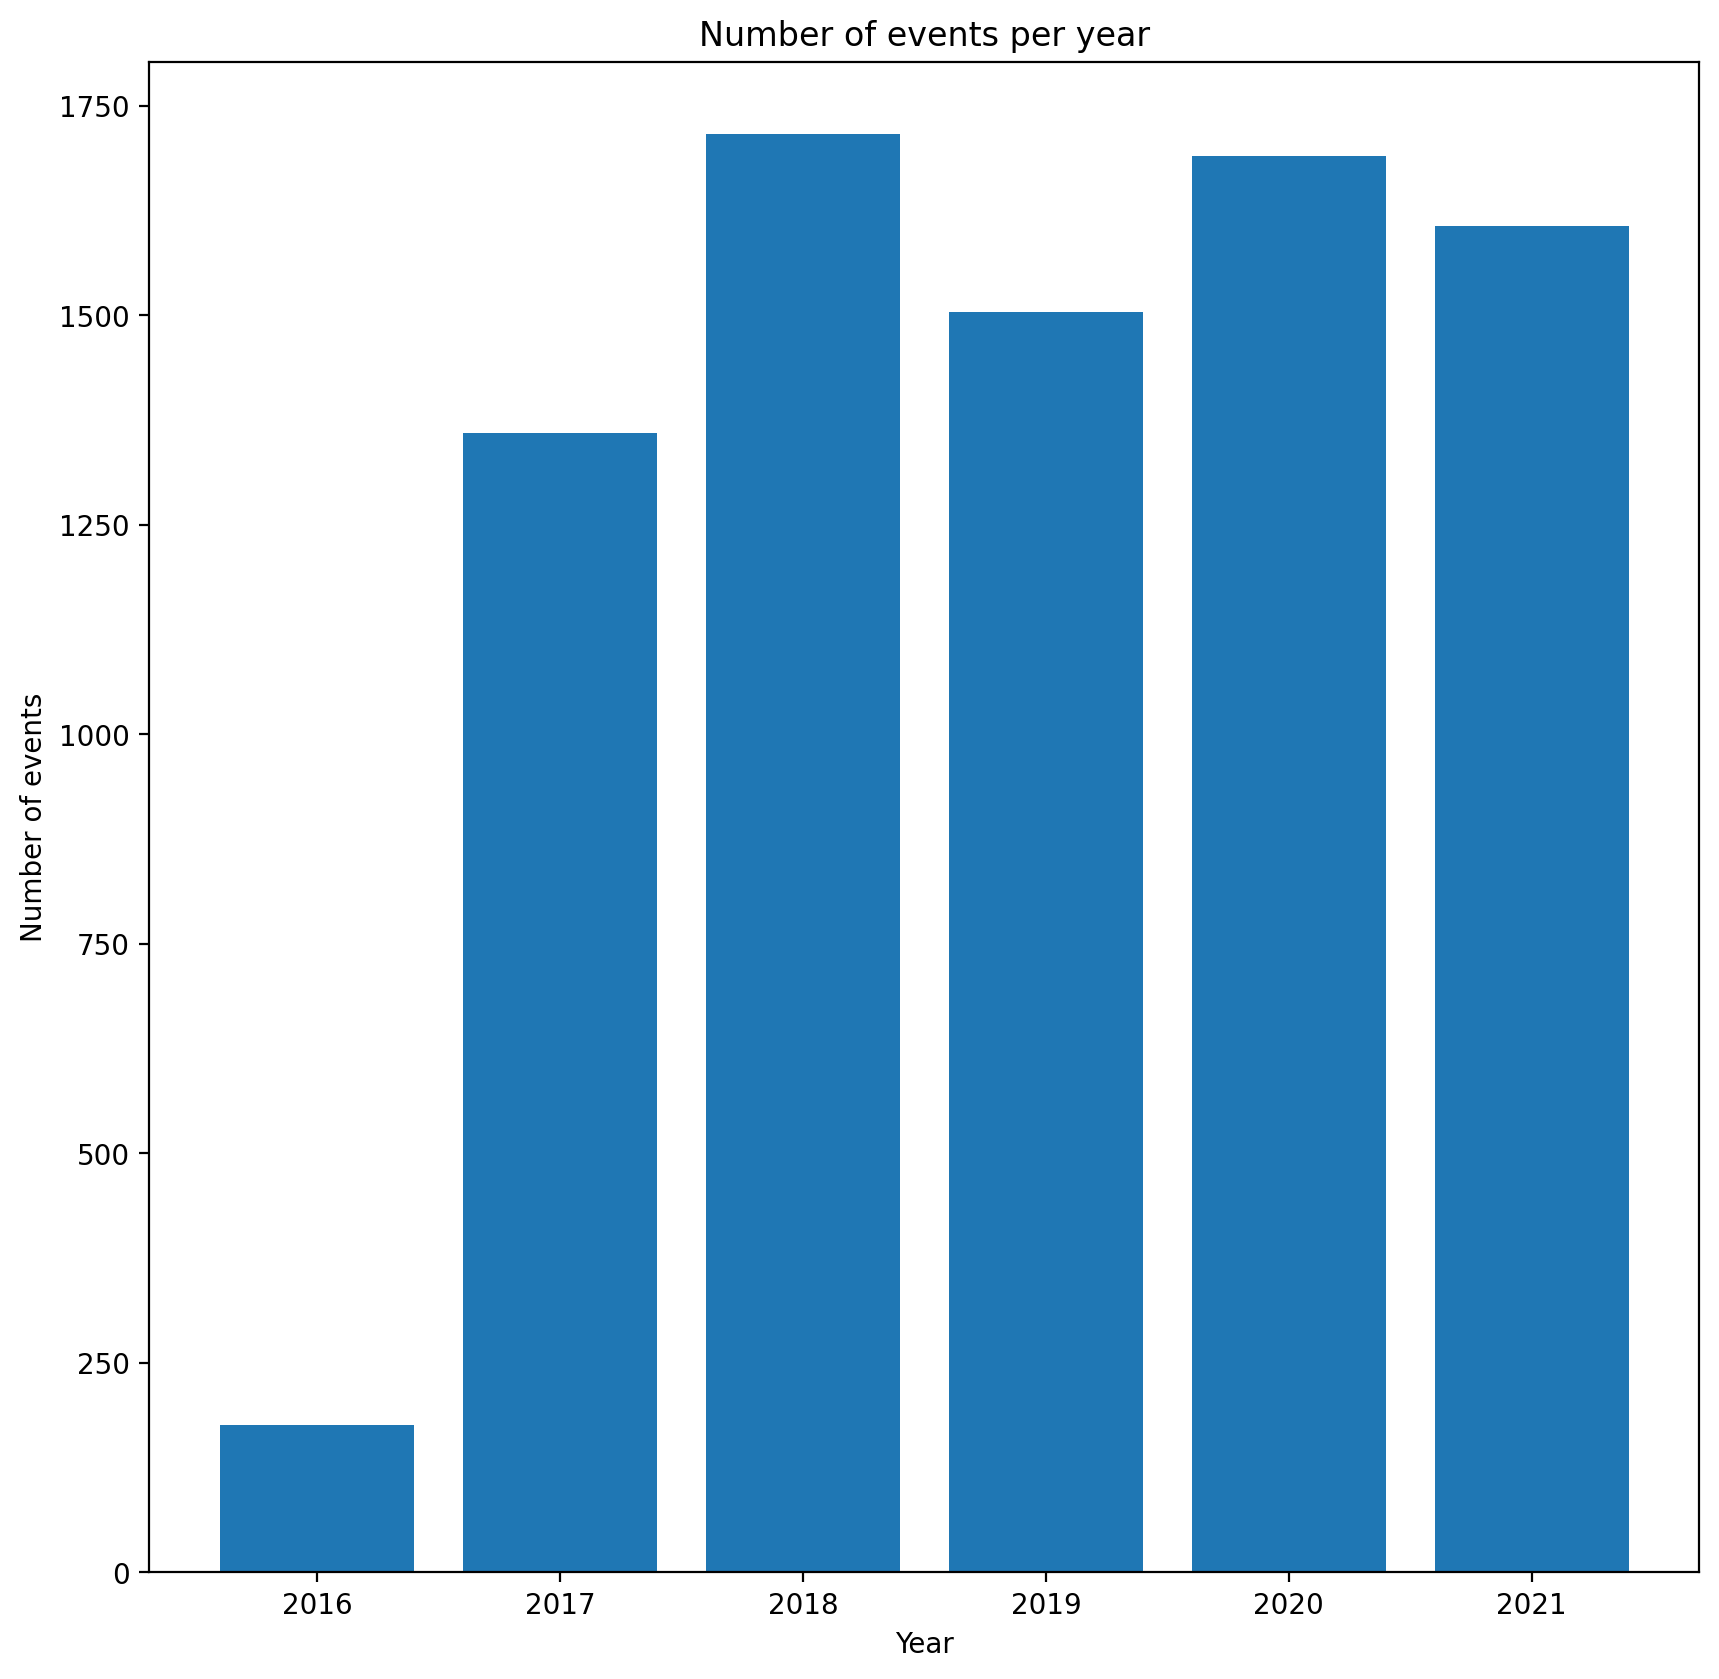
\includegraphics[width=0.45\textwidth]{eventsPerYear.png}
	\caption{Number of events per company}
	\label{fig:eventsPerYear}
\end{figure}
\begin{figure}[ht]
	\centering
	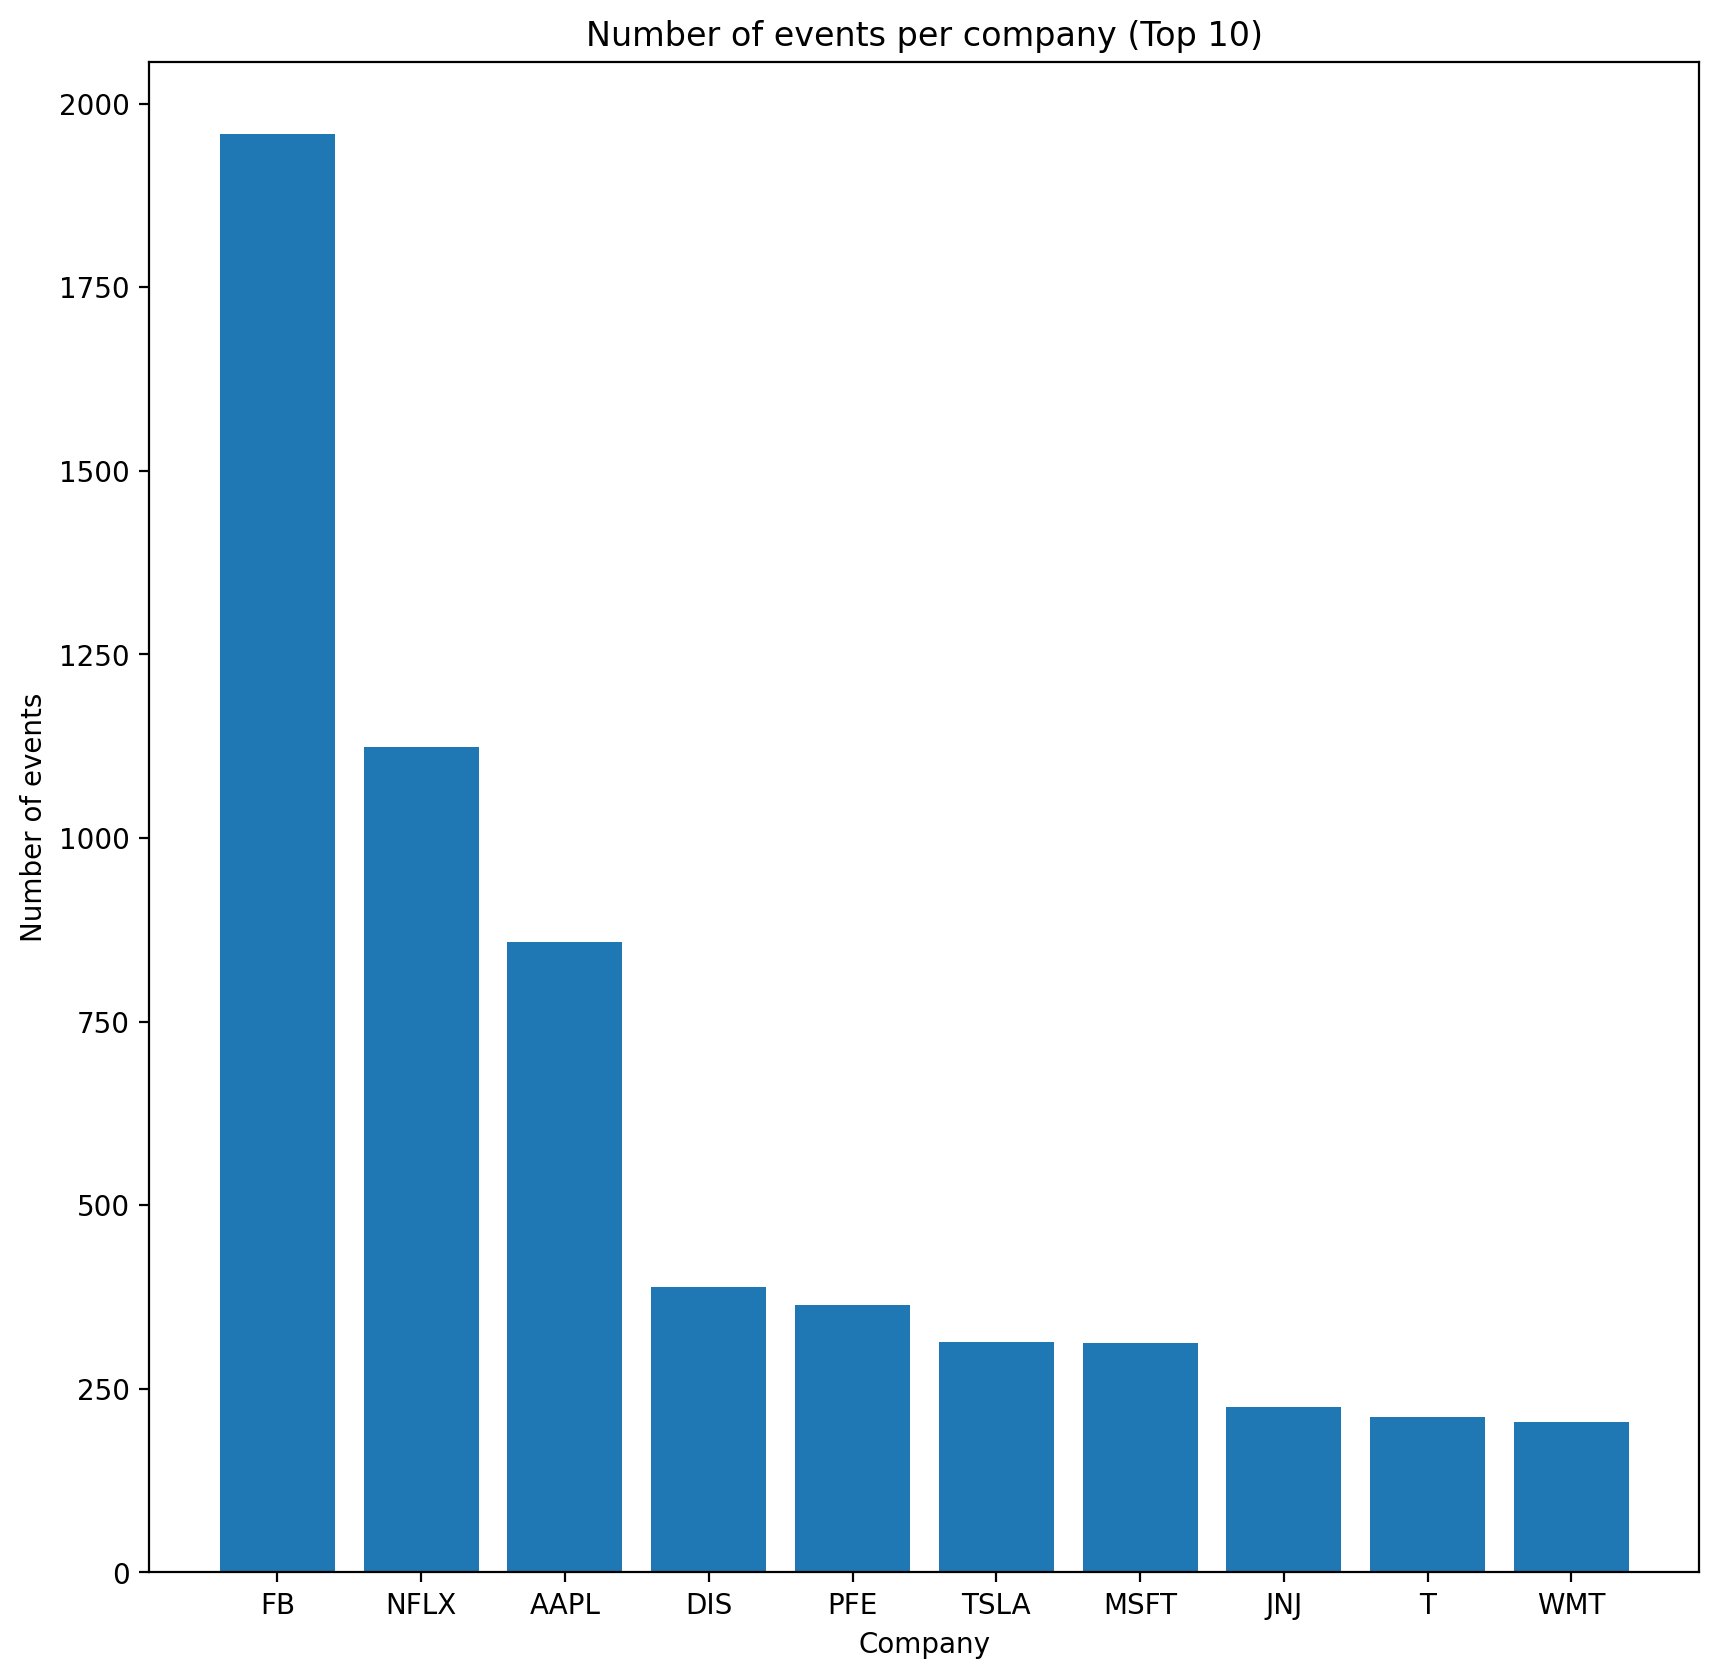
\includegraphics[width=0.45\textwidth]{eventsPerCompany.png}
	\caption{Number of events per company}
	\label{fig:eventsPerCompany}
\end{figure}
\section{Results}
\subsection{Event Study}
\subsubsection{Standard Methodology}
Our event study had the goal of invetsigating if the news releases in our datset were correlated with abnormal returns in stock price. We use the event study methodology as described above, but could not produce signigicant results on a dataset of our size. One possible reason for this is that the number of events is relativevly small.
\subsubsection{Simple Correlation Test}
To confirm our suspicions that our event data in fact had no correlation with price movements, we ran a simple correlation test on a frequecy of news releases for a given company and the absolute acceleration of stock price. Figure \ref{fig:acceleartion} gives an example of this data on Microsoft. The average correlation coefficient over all stocks is 0.035, which means that there is no significant correlation between the news releases and the stock price in our dataset.
\begin{figure}[ht]
	\centering
	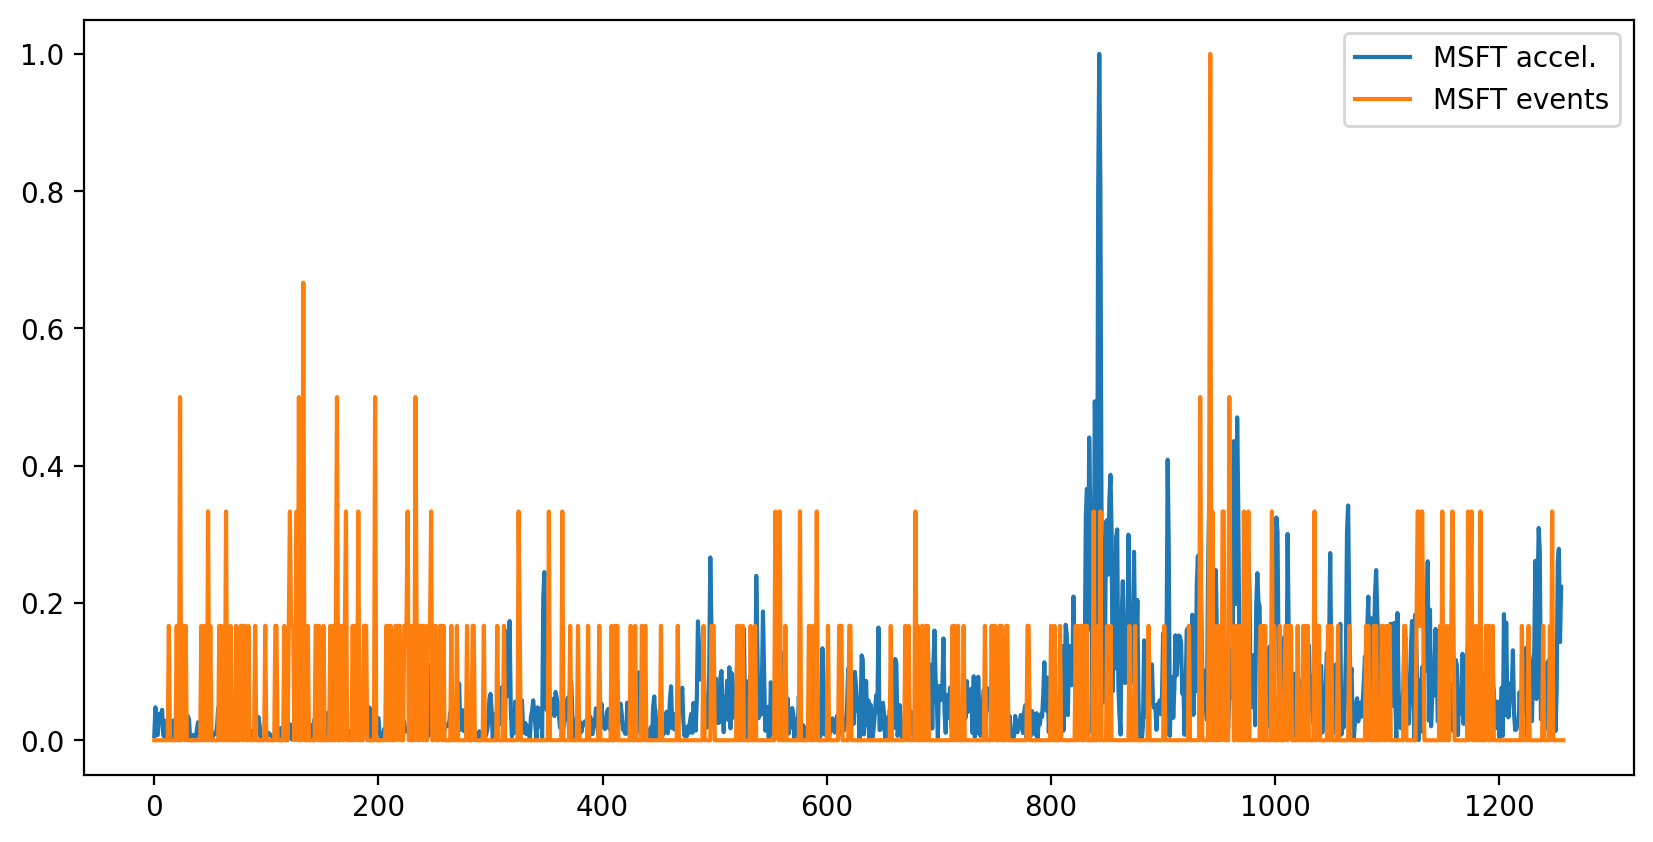
\includegraphics[width=0.45\textwidth]{MSFTevents.png}
	\caption{Acceleration of MSFT vs. News Releases}
	\label{fig:acceleartion}
\end{figure}
\subsection{Inference}
\subsubsection{Format-Correctness Metric}
Suprisingly, GPT-J was always able to retrun a parseable output given our test prompt. \textbf{Give example prompt.} We believe that adding a ``\$'' to the end of the prompt made GPT-J more likely to return a parseable output.
\subsubsection{Price-Accuracy Metric}
Our limited inference method was unable to predict stock prices with any accuracy. In our dataset, a simple linear regression over the past week of stock prices was able to generate a prediction of the next day's price 52\% of the time. By comparision, the GPT-J model was correct 47.5\% of the time. Both of these numbers are not significantly better from a random guess. 
\section{Conclusion}
In conclusion, our study was unable to determine if language models like GPT-J contain any predective power in the stock market. Further study is needed to determine if natural-language-processing based models can be used to predict stock prices.
\subsection{Future Work}
Future work to improve the significane of our results will include:
\begin{itemize}
	\item Including more data sources (news, and other) to increase the number of events we can analyze.
	\item Including more stocks in our analysis.
	\item Varying prompt format.
	\item Increasing the size of our inferernce dataset.
\end{itemize}

% \section*{Acknowledgment}
% The authors would like to thank... 


\bibliographystyle{IEEEtran}
\bibliography{./paper.bib}

\end{document}